\documentclass[12pt,a4paper]{article}
\usepackage[utf8]{vietnam}
\usepackage{graphicx}
\usepackage{xcolor}
\usepackage{wrapfig}
\usepackage{multicol}
\usepackage{fancyhdr}
\usepackage{fancybox}
%Hung
\usepackage{amsmath}
\usepackage{listings}
\usepackage{color}
\definecolor{dkgreen}{rgb}{0,0.6,0}
\definecolor{gray}{rgb}{0.5,0.5,0.5}
\definecolor{mauve}{rgb}{0.58,0,0.82}
 
\lstset{frame=tb,
  language=C++,
  aboveskip=3mm,
  belowskip=3mm,
  showstringspaces=false,
  columns=flexible,
  basicstyle={\small\ttfamily},
  numbers=none,
  numberstyle=\tiny\color{gray},
  keywordstyle=\color{blue},
  commentstyle=\color{dkgreen},
  stringstyle=\color{mauve},
  breaklines=true,
  breakatwhitespace=true,
  tabsize=3
}

\usepackage[unicode]{hyperref}

%endHung


\usepackage[left=2.50cm, right=2.50cm, top=2.00cm, bottom=3.00cm]{geometry}
\pagestyle{fancy}
\fancyhf{}
\fancyhead[LE,RO]{\thepage}

\fancyhead[LO]{\small{Support Vector Machine and Pattern Recognition System}}
\begin{document}
\thispagestyle{empty}
\thisfancypage{
\setlength{\fboxsep}{0pt}
\fbox}{}
\begin{center}
\begin{large}
TRƯỜNG ĐẠI HỌC BÁCH KHOA HÀ NỘI
\end{large} \\
\begin{large}
VIỆN CÔNG NGHỆ THÔNG TIN VÀ TRUYỀN THÔNG
\end{large} \\

\textbf{--------------------  *  ---------------------}\\[1.5cm]

\includegraphics[scale=0.35]{12}
\\
\vspace{2cm}
{\fontsize{25pt}{1}\selectfont Digital Image Processing}\\[1cm]
{\fontsize{15pt}{1}\selectfont Support Vector Machine And Pattern Recognition System}\\[3cm]
\end{center}
\hspace{3cm}
{\fontsize{12pt}{1}
\selectfont Nhóm sinh viên thưc hiện : } \hspace{1pt}
\textbf{\parbox[t]{6cm}{
\selectfont Nguyễn Quang Huy\\[0.3cm]
\selectfont Nguyễn Bá Hùng\\[0.3cm]
\selectfont KSTN - CNTT - K60\\
   }
}\\[16pt]
\vspace{2cm}
\begin{center}
{\fontsize{12pt}{1}\selectfont HÀ NỘI}\\
{\fontsize{12pt}{1}\selectfont \today}
\end{center}
\newpage
\thispagestyle{empty}
\begingroup
\hypersetup{hidelinks}
\tableofcontents
\endgroup 
\newpage
\section{Giới thiệu}
Ngày nay, cùng với sự phát triển của thời kỳ công nghệ 4.0, vấn đề an ninh bảo mật đang được yêu cầu khắt khe tại mọi quốc gia trên thế giới. Các lĩnh vực học máy, trí tuệ nhân tạo, thị giác máy,... là những công nghệ dẫn đầu cho cuộc cách mạng công nghiệp mới, đem lại những ứng dụng vô cùng to lớn, ảnh hưởng đến mọi mặt đời sống xã hội. Một trong những ứng dụng thú vị mà trí tuệ nhân tạo mang lại đó là ứng dụng trong hệ thống nhận dạng, các hệ thống nhận dạng được ra đời với độ tin cậy ngày càng cao. Trong lĩnh vực xử lý ảnh, một trong các bài toán nhận dạng đang rất được quan tâm hiện nay, đó là bài toán nhận dạng khuôn mặt.\par
Có nhiều phương pháp nhận dạng khuôn mặt khác nhau, có thể kể đến như phương pháp PCA(\textit{Principal Component Analysis}), LDA(\textit{Linear Discriminant Analysis}), SVM(\textit{Support Vector Machine}),... Mỗi phương pháp mang lại hiệu quả khác nhau cho từng bài toán cũng như đặc điểm riêng của từng hệ thống nhận dạng khuôn mặt. Phương pháp \textit{Support Vector Machine} ban đầu được tìm ra bởi Vladimir N. Vapnik, phương pháp này ngày càng được sử dụng rộng rãi trong nhiều lĩnh vực, đặc biệt là lĩnh vực phân loại và nhận dạng mẫu. Hệ thống nhận dạng khuôn mặt được đề xuất trong bài viết sử dụng kết hợp hai phương pháp SVM và PCA, qua đó đánh giá thử nghiệm, phân tích ảnh hưởng của SVM đến hệ thống nhận dạng khuôn mặt. Hệ thống nhận dạng khuôn mặt được xây dựng theo một quy trình cụ thể, với tập dữ liệu đầu vào được thu thâp từ các đối tượng trong thế giới thực, hoàn toàn có thể đưa vào sử dụng trong thực tế.    

\newpage
\section{Phương pháp máy vector hỗ trợ - SVM}
Thuật toán SVM ban đầu được tìm ra bởi  Vladimir N. Vapnik và dạng lề mềm được tìm ra bởi Vapnik và Corinna Cortes năm 1995.
Phương pháp này ngày càng được sử dụng rộng rãi trong nhiều lĩnh vực, đặc biệt là
lĩnh vực phân loại và nhận dạng mẫu. \\
Phương pháp SVM ngày càng được sử dụng phổ biến do:
\begin{itemize}
\item SVM rất hiệu quả trong việc giải quyết bài toán với dữ liệu có số chiều lớn.
\item SVM giải quyết tốt vấn đề overfiting, là dữ liệu có nhiễu và tách rời nhóm, hoặc dữ liệu huấn luyện ít.
\item SVM là phương pháp phân lớp nhanh.
\item SVM có hiệu suất tổng hợp tốt và khả năng tính toán cao.
\end{itemize}
Ta khảo sát l mẫu quan sát. Mỗi mẫu quan sát gồm một cặp: một vector $x_i \in R_n$, $i=1,...,l$ với một giá trị xác định $y_i$ mà giá trị của nó xuất phát từ việc gán chủ quan từ người tổ chức dữ liệu. Gọi $P(x,y)$ là hàm phân phối xác xuất  giữa x và y và chưa được xác định tường minh. Cách tổ chức dữ liệu như trên có tính tổng quát cao hơn so với việc chúng ta kết hợp cứng giữa mỗi y với mỗi x, điều này cho phép tính được phân phối của y dựa vào dữ liệu x cho trước. Tuy nhiên, sau phần này a thừa nhận cố định y với x cho trước.\\
\indent Nhiệm vụ của hệ máy học là ánh xạ $x_i \rightarrow y_i$, được định nghĩa từ một tập hợp các ánh xạ $x \rightarrow f(x,a)$, trong đó hàm $f(x,a)$ được gán nhãn bởi các tham số $\alpha$ ($\alpha$ có thể hiệu chỉnh được trong quá trình xử lý trên tập học). Hệ máy học có thể xem như là một hệ quyết định. Với dữ liệu đầu vào là x cho trước, chọn ra một $\alpha$ thích hợp, và kết xuất sẽ là $f(x,a)$. Ta có thể chọn $\alpha$ theo nhiều cách khác nhau, ở đây, chúng ta sẽ tiếp cận theo phương pháp máy học.
\subsection{Giới thiệu}
Do phương pháp SVM liên quan nhiều đến toán học, nên trước khi đi sâu vào nó, chúng ta cùng điểm lại một số kiến thức hình học.
\subsubsection{Khoảng cách từ một điểm tới một siêu mặt phẳng}
Trong không gian 2 chiều, ta biết rằng khoảng cách từ một điểm có toạ độ $(x_0,y_0)$ tới đường thẳng có phương trình $w_{1}x+w_{2}y+b =0$
 được xác định bởi: \\
 \centerline{$\dfrac{|w_{1}x_{0}+w_{2}y_{0}+b|}{\sqrt{w_1^2+w_2^2}}$}\\
 Trong không gian 3 chiều, khoảng cách từ một điểm có tọa độ $(x_0,y_0,z_0)$ tới một mặt phẳng có phương trình $w_{1}x+w_{2}y+w_3z+b = 0$ được xác định bởi:\\
 \centerline{$\dfrac{|w_{1}x_{0}+w_{2}y_{0}+w_{3}z_{0} +b|}{\sqrt{w_1^2+w_2^2+w_3^2}}$}\\
 Hơn nữa, nếu ta bỏ dấu trị tuyệt đối ở tử số, chúng ta có thể xác định được điểm đó nằm về phía nào của đường thẳng hay mặt phẳng đang xét. Những điểm làm cho biểu thức trong dấu giá trị tuyệt đối mang dấu dương nằm về cùng 1 phía (tôi tạm gọi đây là phía dương của đường thẳng), những điểm làm cho biểu thức trong dấu giá trị tuyệt đối mang dấu âm nằm về phía còn lại (tôi gọi là phía âm). Những điểm nằm trên đường thẳng/măt phẳng sẽ làm cho tử số có giá trị bằng 0, tức khoảng cách bằng 0.\\
 Việc này có thể được tổng quát lên không gian nhiều chiều: Khoảng cách từ một điểm (vector) có toạ độ $x_0$ tới siêu mặt phẳng (hyperplane) có phương trình $w^Tx+b=0$ được xác định bởi:\\
 \centerline{$\dfrac{|w^Tx_0+b|}{||w||_2}$}\\
 với $||w||_2 = \sqrt{\sum_{i=1}^{d}w_i^2 }$ với d là số chiều của không gian.\\
 \subsubsection{Nhắc lại bài toán phân chia hai classes}
 Giả sử có hai class khác nhau được mô tả bởi các điểm trong không gian nhiều chiều, hai classes này phân chia tuyên tính, tức là tồn tại một siêu phẳng phân chia chính xác hai classes đó. Hãy tìm một mặt phẳng phân chia hai classes đó, tức tất cả các điểm thuộc một class nằm về cùng một phía của siêu mặt phẳng đó và ngược phía với toàn bộ các điểm thuộc class còn lại. Chúng ta đã biết rằng, thuật toán PLA có thể làm được việc này nhưng nó có thể cho chúng ta vô số nghiệm như Hình 1 dưới đây:
 \begin{center}
 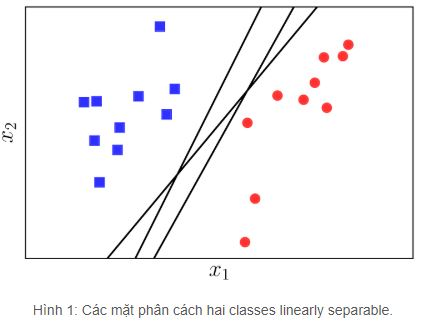
\includegraphics[scale=1]{img/img1}
 \end{center}
 Câu hỏi đặt ra là: trong vô số các mặt phân chia đó, đâu là mặt phân chia tốt nhất theo một tiêu chuẩn nào đó? Trong ba đường thẳng minh họa trong Hình 1 phía trên, có hai đường thẳng khá lệch về phía class hình tròn đỏ. Điều này có thể khiến cho lớp màu đỏ không vui vì lãnh thổ xem ra bị lấn nhiều quá. Liệu có cách nào để tìm được đường phân chia mà cả hai classes đều cảm thấy công bằng và hạnh phúc nhất hay không?\\Chúng ta cần tìm một tiêu chuẩn để đo sự hạnh phúc của mỗi class. Hãy xem Hình 2 dưới đây:
 \begin{center}
 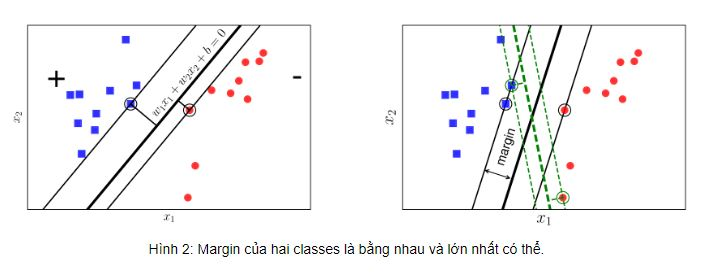
\includegraphics[scale=1]{img/img2}
 \end{center}
Nếu ta định nghĩa mức độ hạnh phúc của một class tỉ lệ thuận với khoảng cách gần nhất từ một điểm của class đó tới đường/mặt phân chia, thì ở Hình 2 trái, class tròn đỏ sẽ không được hạnh phúc cho lắm vì đường phân chia gần nó hơn class vuông xanh rất nhiều. Chúng ta cần một đường phân chia sao cho khoảng cách từ điểm gần nhất của mỗi class (các điểm được khoanh tròn) tới đường phân chia là như nhau, như thế thì mới công bằng. Khoảng cách như nhau này được gọi là margin (lề).\\
Đã có công bằng rồi, chúng ta cần văn minh nữa. Công bằng mà cả hai đều kém hạnh phúc như nhau thì chưa phải là văn mình cho lắm.\\
Chúng ta xét tiếp Hình 2 bên phải khi khoảng cách từ đường phân chia tới các điểm gần nhất của mỗi class là như nhau. Xét hai cách phân chia bởi đường nét liền màu đen và đường nét đứt màu lục, đường nào sẽ làm cho cả hai class hạnh phúc hơn? Rõ ràng đó phải là đường nét liền màu đen vì nó tạo ra một margin rộng hơn.\\
Việc margin rộng hơn sẽ mang lại hiệu ứng phân lớp tốt hơn vì sự phân chia giữa hai classes là rạch ròi hơn. Việc này, sau này các bạn sẽ thấy, là một điểm khá quan trọng giúp Support Vector Machine mang lại kết quả phân loại tốt hơn so với Neural Network với 1 layer, tức Perceptron Learning Algorithm.\\
Bài toán tối ưu trong Support Vector Machine (SVM) chính là bài toán đi tìm đường phân chia sao cho margin là lớn nhất. Đây cũng là lý do vì sao SVM còn được gọi là Maximum Margin Classifier. Nguồn gốc của tên gọi Support Vector Machine sẽ sớm được làm sáng tỏ.
\subsection{SVM tuyến tính}
\subsubsection{SVM trong trường hợp tập mẫu có thể phân cách tuyến tính}
\indent Máy học được huấn luyện trên dữ liệu có thể phân loại tuyến tính, đây là trường hợp đơn giản nhất của hệ máy học. Gán nhãn dữ liệu huấn luyện ${x_i,y_i}$ với $i=1,2,...,n$, $x_i \in R^d$, $y_i \in {-1,1}$. Giả sử có các siêu mặt phẳng phân loại mẫu dương với mẫu âm (gọi là "siêu mặt phân cách"). Điểm x nằm trên siêu mặt phẳng thỏa mãn phương trình $wx+b=0$, trong đó w là pháp tuyến của siêu mặt phẳng phân cách, $|b|$ là khoảng cách từ siêu mặt đến gốc tọa độ, và $||w||$ là độ lớn (Euclide) của w.\\
\indent Để dễ hình dung, chúng ta cùng xét trường hợp trong không gian hai chiều dưới đây.  
\begin{center}
    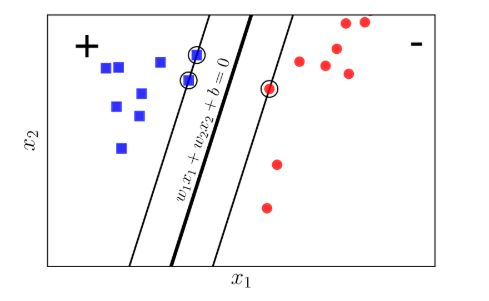
\includegraphics[scale=1]{img/img3}
\end{center}
\indent Giả sử rằng các điểm vuông xanh thuộc class 1, các điểm tròn đỏ thuộc class -1 và mặt $w^Tx+b=w_1x_1+w_2x_2+b=0$ là mặt phân chia giữa hai classes (Hình trên). Hơn nữa, class 1 nằm về phía dương, class -1 nằm về phía âm của mặt phân chia. Nếu ngược lại, ta chỉ cần đổi dấu của $w$ và $b$. Chú ý rằng chúng ta cần đi tìm các hệ số $w$ và $b$.\\
\indent Ta quan sát thấy một điểm quan trọng sau đây: với cặp dữ liệu $(x_n,y_n)$ bất kỳ, khoảng cách từ điểm đó tới mặt phân chia là: \\
\centerline{$\dfrac{y_n(w^Tx_n+b)}{||w||_2}$}\\
\indent Điều này có thể dễ nhận thấy vì theo giả sử ở trên, $y_n$ luôn cùng dấu với phía của $x_n$. Từ đó suy ra $y_n$ cùng dấu với $(w^Tx_n+b)$, và tử số luôn là 1 số không âm.\\
Với mặt phần chia như trên, margin được tính là khoảng cách gần nhất từ 1 điểm tới mặt đó (bất kể điểm nào trong hai classes):\\
\centerline{$margin = min_{n}\dfrac{y_n(w^Tx_n+b)}{||w||_2}$}\\
\indent Bài toán tối ưu trong SVM chính là bài toán tìm $w$ và $b$ sao cho margin này đạt giá trị lớn nhất:\\
\centerline{$(w,b) = argmax_{w,b}\{min_n\dfrac{y_n(w^Tx_n+b)}{||w||_2}\} = argmax_{w,b} = argmax_{w,b}\{\dfrac{1}{||w||_2}min_n y_n(w^Tx_n+b)\}$}\\
\indent Việc giải bài toán này sẽ rất phức tạp, nhưng các bạn sẽ thấy có cách đưa nó về bài toán đơn giản hơn.\\
\indent Nhận xét quan trọng nhất là nếu ta thay vector hệ số $w$ bởi $kw$ và $b$ bởi $kb$ là một hằng số dương thì mặt phân chia không thay đổi, tức khoảng cách từ từng điểm đến mặt phân chia không đổi, tức margin không đổi. Dựa trên tính chất này, ta có thể giả sử:\\
\centerline{$y_n(w^Tx_n+b)=1$}\\
với những điểm gần mặt phân chia nhất, như hình dưới đây:
\begin{center}
    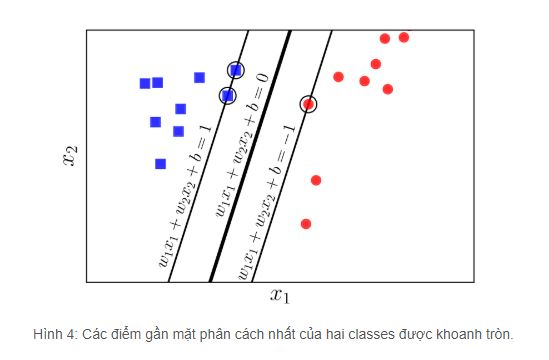
\includegraphics[scale=1]{img/img4}
\end{center}
Như vậy, với mọi n, ta có:\\
\centerline{$y_n(w^Tx_n+b) \geq 1$}\\
Vậy bài toán tối ưu $(1)$ có thể đưa về bài toán tối ưu có ràng buộc sau đây:\\
\centerline{$(w,b) = argmax_{w,b}\dfrac{1}{||w||_2}$}\\
\centerline{với $y_n(w^Tx_n+b) \geq 1$, với mọi $n=1,2,...,l$}\\
Và chúng ta đưa về:\\
\centerline{$(w,b)=argmin_{w,b}\dfrac{1}{2}||w||^2_2$}\\
\centerline{$y_n(w^Tx_n+b) -1 \geq 0$, với mọi $n=1,2,...,l$\ \ \ (3)}\\
\indent Ở đây chúng ta đã lấy nghịch đảo hàm mục tiêu, bình phương nó để được một hàm khả vi, và nhân với $\dfrac{1}{2}$ để biểu thức đạo hàm đẹp hơn.\\
\indent Để giải quyết bài toán này, chúng ta có thể dùng hàm Lagrange bởi vì các lý do sau. Thứ nhất, ràng buộc bất đẳng thức (3) sẽ được thay thế bằng ràng buộc trên hệ số nhân Lagrange để dễ làm việc hơn. Thứ hai, dữ liệu huấn luyện sẽ chỉ xuất hiện dưới dạng phép nhân vô hướng giữa các vector, điều này cho phép tổng quát hóa trong trường hợp phi tuyến.\\
Với ràng buộc bất đẳng thức (3) có vế trái $\geq 0 $ thì ta nhân với hệ số Lagrange $\alpha_i > 0$ và phương trình ràng buộc sau khi nhân với hệ số Lagrange thì sẽ bị trừ khỏi hàm mục tiêu. Với các ràng buộc là đẳng thức thì hệ số nhân Lagrange không bị ràng buộc. Khi đó hàm Lagrange có dạng sau:\\
\centerline{$L_p = \dfrac{1}{2} ||w||^2 - \sum_{i=1}^l \alpha_iy_i(wx_i+b)+\sum_{i=1}^l\alpha_i$\ \ \ \ (4)}\\
\indent Mục tiêu của chúng ta là phải cực tiểu $L_p$ theo pháp tuyến w và b, và đạo hàm của $L_p$ triệt tiêu với mọi $\alpha_i\geq0$(gọi tập ràng buộc này là $C_1$). Hay nói cách khác là giải bài toán đối ngẫu đó tìm cực đại $L_p$ với điều kiện đạo hàm của $L_p$ triệt tiêu với $w,b$ và cũng với ràng buộc $\alpha_i \geq 0$ (gọi tập ràng buộc này là $C_2$).\\
Đạo hàm $L_p$ triệt tiêu với $w$ và $b$ ta có các điều kiện: $w=\sum_{i=1}^l\alpha_ix_iy_i =0$\ \ \ \ (5)\\
Vì đây là các ràng buộc tuyến tính nên: $\sum_{i=1}^{l}\alpha_iy_i=0$\ \ \ \ (6) \\
Thay vào (4) ta được: $L_D = \sum_i \alpha_i - \dfrac{1}{2}\sum_{i,j}\alpha_i\alpha_jx_ix_jy_iy_j$ \ \ \ (7)\\
Trong trường hợp tuyến tính và có thể phân loại, việc huấn luyện SVM là làm cực đại $L_D$ theo $\alpha_i > 0$ với ràng buộc (6), với lời giải được tính theo (5). Khi đó, các mẫu thỏa điều kiện $\alpha_i > 0$ được gọi là "vector hỗ trợ - SVM" và nằm trên một trong hai siêu mặt âm hoặc dương (như đã nói ở trên). Các điểm dữ liệu còn lại có $\alpha_i=0$ và nằm trên mặt âm hoặc dương thỏa mãn trường hợp dấu bằng xảy ra của (3), hoặc chúng nằm về một phía của mặt âm hoặc dương trong trường hợp thỏa mãn bất đẳng thức (3). Khi đó, các vector hỗ trợ là các thành phần tới hạn của tập huấn luyện. Nếu mọi điểm huấn luyện khác bị loại bỏ và việc huấn luyện được lặp lại thì các siêu mặt phân cách đã tìm thấy không bị thay đổi.\\
\indent Nếu số thuộc tính của các mẫu dữ liệu là lớn, chúng ta có thể đơn giản hóa bằng cách chuyển bài toán với điều kiện Karush-Kuhn-Tucker, tương đương với phương trình Lagrage dạng kép. Điều kiện Karush-Kuhn-Tucker có vai trò quan trọng trong bài toán tối ưu ràng buộc. Với bài toán trên, điều kiện Karush-Kuhn-Tucker có thể phát biểu như sau: \\
\centerline{$\dfrac{\partial}{\partial w_v}L_p = w_v - \sum_i \alpha_iy_ix_{iv} = 0$ với v=1,..,d}\\
\centerline{$\dfrac{\partial}{\partial b}L_p = -\sum_i\alpha_iy_i=0$}\\
\centerline{$y_i(wx_i+b)-1 \geq 0$ với i=1,...,l}\ \ \ (8)\\
\centerline{$\alpha_i \geq 0$ với mọi i}\\
\indent Giải bài toán này ta tìm được $\alpha$ và từ đó tính được w theo công thức (5). Tính b, vận dụng điều kiện KKT cho bài toán gốc, ta có được:\\
\centerline{$\alpha_i[y_i(wx_i+b)-1]=0$ với i =1,2,..,l}\\
Do đó, với mỗi i ta có 2 trường hợp:\\
\begin{itemize}
    \item $\alpha_i = 0$: Trong trường hợp này $y_i(wx_i+b)-1>0$ suy ra $x_i$ không nằm trên siêu phẳng âm hay dương. Vì $\alpha_i=0$ nên $x_i$ không tham gia vào việc cấu trúc w theo công thức (8).Những $x_i$ này là không cần thiết và có thể được bỏ đi mà không ảnh hưởng đến w.
    \item $\alpha_i>0$: trong trường hợp này $y_i(wx_i+b)-1=0$ suy ra $x_i$ nằm trên siêu phẳng biên âm hay dương, $x_i$ được gọi là support vector và tham gia vào việc tính toán w. Thông thường số lượng support vector nhỏ hơn nhiều so với số lượng mẫu.
\end{itemize}
Do vậy, để tính b ta chỉ cần chọn một giá trị i mà khi đó $\alpha_i>0$, lúc đó ta lần lượt tính các giá trị của ngưỡng b và lấy giá trị trung bình của ngưỡng b thu được đó.
\subsubsection{SVM trong trường hợp tập mẫu không thể phân cách tuyến tính}
Trường hợp tập mẫu có thể phân cách tuyến tính chỉ là một trường hợp đặc biệt. Trong trường hợp tổng quát, tập mẫu là tập không thể phân cách tuyến tính bằng một siêu phẳng.
\newpage
\begin{center}
    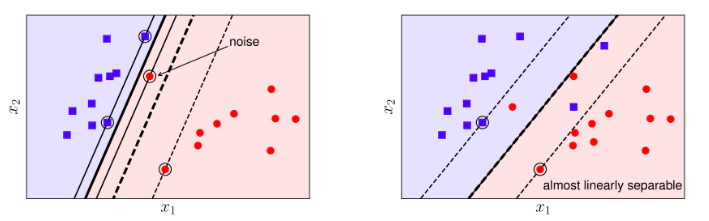
\includegraphics[scale=0.7]{img/img5.png}

\end{center}
Có hai trường hợp dễ nhận thấy SVM làm việc không hiệu quả hoặc thậm chí không làm việc:
\begin{itemize}
    \item Trường hợp 1: Dữ liệu vẫn phân chia tuyến tính như Hình đầu nhưng có một điểm nhiễu của lớp tròn đỏ ở quá gần so với lớp vuông xanh. Trong trường hợp này, nếu ta sử dụng SVM thuần thì sẽ tạo ra một margin rất nhỏ. Ngoài ra, đường phân lớp nằm quá gần lớp vuông xanh và xa lớp tròn đỏ. Trong khi đó, nếu ta hy sinh điểm nhiễu này thì ta được một margin tốt hơn rất nhiều được mô tả bởi các đường nét đứt. SVM thuần vì vậy còn được coi là nhạy cảm với nhiễu (sensitive to noise).
    \item Dữ liệu không phân tách tuyến tính nhưng gần phân chia tuyến tính như Hình thứ 2. Trong trường hợp này, nếu ta sử dụng SVM thuần thì rõ ràng bài toán tối ưu là không khả thi, tức tập khả thi của nó là một tập rỗng, vì vậy bài toán tối ưu SVM trở nên vô nghiệm. Tuy nhiên, nếu ta lại chịu hy sinh một chút những điểm ở gần biên giữa hai lớp, ta vẫn có thể tạo được một đường phân chia khá tốt như đường nét đứt đậm. Các đường support đường nét đứt mảnh vẫn giúp tạo được một margin lớn cho bộ phân lớp này. Với mỗi điểm nằm lần sang phía bên kia của các đường suport (hay đường margin, hoặc đường biên) tương ứng, ta gọi điểm đó rơi vào vùng không an toàn. Chú ý rằng vùng an toàn của hai classes là khác nhau, giao nhau ở phần nằm giữa hai đường support.
\end{itemize}
\indent Trong cả hai trường hợp trên, margin tạo bởi đường phân chia và đường nét đứt mảnh còn được gọi là soft margin (biên mềm). Cũng theo cách gọi này, SVM thuần còn được gọi là Hard Margin SVM (SVM biên cứng).\\
\indent Trong mục này, chúng ta sẽ tiếp tục tìm hiểu một biến thể của Hard Margin SVM có tên gọi là Soft Margin SVM.\\
\indent Như đã đề cập phía trên, để có một margin lớn hơn trong Soft Margin SVM, chúng ta cần hy sinh một vài điểm dữ liệu bằng cách chấp nhận cho chúng rơi vào vùng không an toàn. Tất nhiên, chúng ta phải hạn chế sự hy sinh này, nếu không, chúng ta có thể tạo ra một biên cực lớn bằng cách hy sinh hầu hết các điểm. Vậy hàm mục tiêu nên là một sự kết hợp để tối đa margin và tối thiểu sự hy sinh.\\
\indent Giống như với Hard Margin SVM, việc tối đa margin có thể đưa về việc tối thiểu $||w||_2^2$. Để xác định sự hy sinh, chúng ta cùng theo dõi Hình dưới đây:\\
\begin{center}
    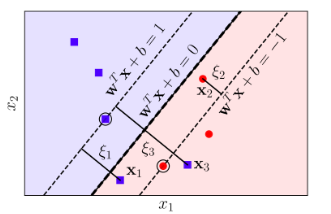
\includegraphics[scale=1.0]{img/img6.png}
\end{center}
\indent Ở đây mình sẽ giới thiệu các biến slack $\xi_n$. Với những điểm nằm trong vùng an toàn, $\xi_n$. Những điểm nằm trong vùng không an toàn nhưng vẫn đúng phía so với đường phân chia tương ứng với các $0 < \xi_n < 1$, ví dụ $x_2$. Những điểm nằm ngược phía với class của chúng so với đường boundary ứng với các $\xi_n >1$, ví dụ như $x_1$ và $x_3$.
Với mỗi điểm $x_n$ trong tập toàn bộ dữ liệu huấn luyện, ta giới thiệu thêm một biến đo sự hi sinh $\xi_n$.Biến này còn được gọi là slack variable. Với những điểm $x_n$ nằm trong vùng an toàn, $\xi_n = 0$. Với mỗi điểm nằm trong vùng không an toàn như $x_1, x_2 hay x_3$, ta có $\xi_i > 0$. Nhận thấy rằng nếu $y_i = \pm{1}$ là nhãn của $x_i$ trong vùng không an toàn thì $\xi_i = |w^Tx_i + b - y_i|$\\
Trong bài toán tối ưu SVM thuần: \\
\begin{center}
$(w,b) = argmin_{w,b}\dfrac{1}{2}||w||_2^2$\\
với: $y_n(w^Tx_n +b) \geq 1$ với mọi $n=1,2,...,N$
\end{center}
\indent Với Soft Margin SVM, hàm mục tiêu sẽ có thêm một số hạng nữa giúp tối thiểu sự hy sinh. Từ đó ta có hàm mục tiêu:\\
\centerline{$\dfrac{1}{2}||w||_2^2 + C\sum_{n=1}^N\xi_n$}\\
Trong đó C là hằng số dương và $\xi = [\xi_1,\xi_2,...,\xi_N]$\\
\indent Hằng số C được dùng để điều chỉnh tầm quan trọng giữa margin và sự hi sinh. Hằng số này được xác định từ trước bởi người lập trình.\\
Điều kiện ràng buộc sẽ có thay đổi một chút so với SVM thuần. Với mỗi cặp dữ liệu $(x_n,y_n)$ thay vì ràng buộc cứng $y_n(^Tx_n+b) \geq 1$ chúng ta sẽ có ràng buộc mềm: \\
$y_n(w^Tx_n+b) \geq 1 - \xi_n \rightarrow 1-\xi_n - y_n(w^Tx_n +b) \leq 0$ với mọi $n=1,2,...,n$ \\
Và ràng buộc phụ $\xi_n \geq 0$, với mọi n =1,2,...,N \\ 
\indent Tóm lại, ta sẽ có bài toán tối ưu ở dạng chuẩn cho Soft-margin SVM:
\begin{center}
    $(w,b,\xi) = argmin_{w,b,\xi}\dfrac{1}{2}||w||_2^2 + C\sum_{n=1}^N\xi_n$\\
    Với điều kiện: $1-\xi_n - y_n(w^Tx_n+b) \leq 0$, với n=1,2,3,...,N \\
    và $\xi_n \geq 0$
\end{center}
Bây giờ ta sẽ phân tích chi tiết và cách giải bài toán trên: \\
Bài toán đối ngẫu của bài toán trên sẽ là:
Cực đại $\phi(\alpha,\nu)$ dựa trên điều kiện $\alpha \in R^N, \nu\in R^N, \alpha \geq 0, \nu \geq 0$\\
\centerline{$\phi(\alpha, \nu) = inf{\dfrac{1}{2}||w||_2^2+C\sum_{i=1}^N\xi_i - \sum_{i=1}^N\alpha_i[y_i(wx_i+b)-1+\xi_i] - \sum_{i=1}^N \nu_i\xi_i}$}\\
Cũng theo điều kiện Fermat cực tiểu của: \\
\indent $L(w,b,\xi) = \dfrac{1}{2}||w||_2^2+C\sum_{i=1}^N\xi_i - \sum_{i=1}^N\alpha_i[y_i(wx_i+b)-1+\xi_i] - \sum_{i=1}^N \nu_i\xi_i$\\
Xảy ra tại w,b,$\xi$ sao cho: \\ 
\indent  $\dfrac{\partial L(w,b,\xi)}{\partial w} = w - \sum_{i=1}^N \alpha_ix_iy_i = 0 \rightarrow w = \sum_{i=1}^N\alpha_ix_iy_i$\\
\indent  $\dfrac{\partial L(w,b,\xi)}{\partial b} = -\sum_{i=1}^N \alpha_iy_i=0$\\
\indent $\dfrac{\partial L(w,b,\xi)}{\partial \xi_i} = C- \alpha_i - \nu_i =0 \rightarrow 0 \leq \alpha_i \leq C$\\
Lúc đó giá trị cực tiểu của L là:\\
\indent $L_0(w,b,\xi) = \dfrac{1}{2}||w||^2 + C\sum_{i=1}^N\xi_i - \sum_{i=1}^N \alpha_i[y_i(wx_i+b)-1+\xi_i]-\sum_{i=1}^N\nu_i\xi_i$\\
\indent $L_0(w,b,\xi) = \sum_{i=1}^N\alpha_i - \dfrac{1}{2}\sum_{i=1}^N\sum_{i=1}^N\alpha_i\alpha_jx_ix_jy_iy_j$\\
Như vậy, bài toán đối ngẫu được viết lại thành tìm cực đại của:\\
\indent $F(\alpha) =\sum_{i=1}^N\alpha_i - \dfrac{1}{2}\sum_{i=1}^N\sum_{i=1}^N\alpha_i\alpha_jx_ix_jy_iy_j$\\
Dựa trên điều kiện: $0\leq \alpha_i \leq C, i=0,1,2,...,l; \sum_{i=1}^N\alpha_iy_i=0$\\
\indent Bài toán natf hoàn toàn giống bài toán mẫu có thể phân tách tuyến tính với điều kiện mở rộng $\alpha_i \leq C$. Giải bài toán này ta tìm được các thành phần của công thức. Từ đó ta tính được w, trong đó $x_i$ là các support vector và các vector lỗi ứng với $0 \leq \alpha_i \leq C$\\
Để tìm b, sử dụng điều kiện Karush-Kuhn-Tucker cho bài toán gốc, ta có:\\
\indent $\alpha_i[y_i(wx_i+b)-1+\xi_i] = 0$\\
\indent $\nu_i\xi_i=0$\\
Chọn một giá trị $\alpha_i$ sao cho $0<\alpha_i<C$ lúc đó \indent $y_i(wx_i+b)-1+\xi_i=0$ để điều kiện xảy ra.\\
\indent Do $C-\alpha_i - \nu_i =0$ suy ra $\nu_i > 0$ nên có thêm điều kiện $\xi_i$ để bất đẳng thức xảy ra. Lúc đó ta có thể tính được:\\
$b = y_i -wx_i$\\
\indent Như vậy, ta đã tìm được siêu phẳng phân chia một tập dữ liệu không thể phân chia tuyến tính. Siêu phẳng này được gọi là siêu phẳng khoảng cách phân hoạch mềm.
\subsubsection{SVM cho vấn đề nhận dạng đa lớp}
Trong các phần trên đã đề cập đến vấn đề SVM nhận dạng cho hai lớp, $y_i= {-1,1}$. Phương pháp SVM chỉ được xây dựng trên nền tảng nhận dạng 2 lớp, bắt đầu từ lý thuyết học thống kê. Đối với nhận dạng đa lớp, ta có thể kết hợp nhiều SVM hai lớp lại với nhau từng đôi một, ở đây mình sẽ trình bày chến lược One vs All.\\
\indent Giả sử cần phải nhận dạng s lớp thì sử dụng s SVM. SVM thứ i sẽ phân biệt với lớp i với lớp còn lại (nếu i là lớp 1 thì lớp còn lại là lớp -1). Một mẫu thử x sẽ được cho kiểm tra trên s SVM này. Hàm nhận dạng của SVM thứ i nào cho ra kết quả bé nhất thì mẫu thử thứ x thuộc lớp thứ i đó.
\begin{figure}
    \centering
    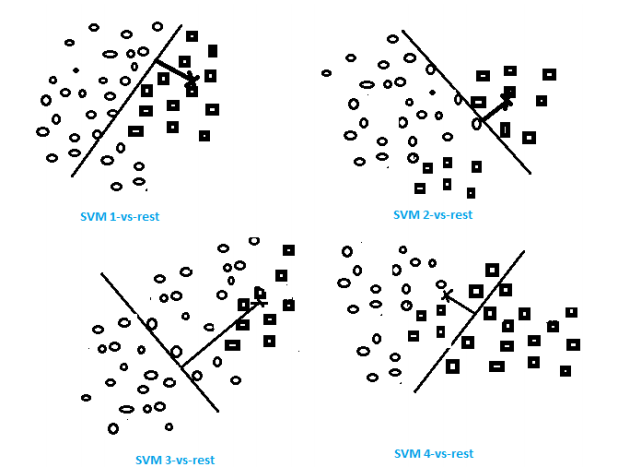
\includegraphics[scale=0.7]{img/img7.png}
    \caption{Mẫu cần nhận dạng là SVM 2-vs-rest vì có giá trị bé nhất}
    \label{fig:my_label}
\end{figure}

\section{Hệ thống nhận dạng}
Hệ thống nhận dạng là một hệ thống tự động nhằm mục đích phân loại mẫu đầu vào thành một lớp cụ thể. Hệ thống tiến hành hai nhiệm vụ liên tiếp: (1) phân tích(hoặc mô tả) trích xuất đặc trưng từ mẫu đang được học và (2) phân lớp(hoặc nhận dạng) đối tượng sử dụng một số đặc trưng được trính xuất trong nhiệm vụ (1). \par 
Sơ đồ phân lớp dựa trên các mẫu đã được phân loại trong tập dữ liệu huấn luyện. Quá trình huấn luyện là quá trình học có giám sát, là thuật toán dự đoán đầu ra của một dữ liệu mới dựa trên các cặp đầu vào và nhãn lớp đã biết từ trước, phân lớp dựa trên các đặc tính của đối tượng. Phân tích mẫu cho phép sử dụng các đặc tính để mô tả và đại diện cho đối tượng thay vì tất cả các thuộc tính của đối tượng. \par 
\subsection{Sơ đồ khối hệ thống nhận dạng}
\begin{center}
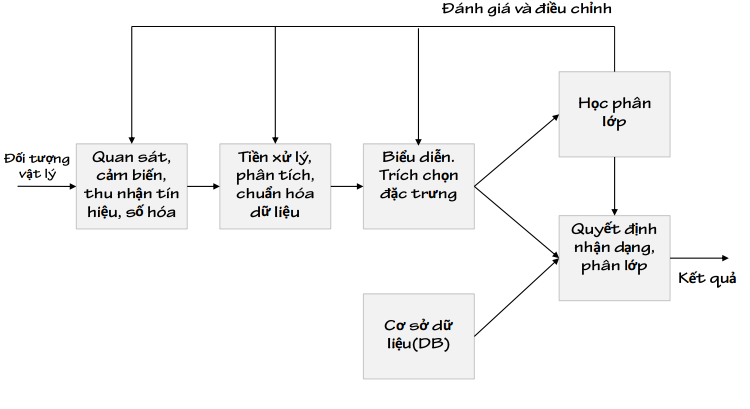
\includegraphics[scale=0.8]{23.png}\\
\textit{Sơ đồ chung của hệ thống nhận dạng}
\end{center}
\par 

\subsubsection{Thu thập dữ liệu}
Ảnh được chụp từ camera, qua quá trình số hóa ảnh(lấy mẫu tín hiệu và lượng tử hóa giá trị) thu được ảnh số. 
\subsubsection{Tiền xử lý ảnh}
Tiền xử lý ảnh nhằm mục đích lọc nhiễu, nâng cao chất lượng ảnh, chuẩn hóa kích cỡ ảnh. Nâng cao chất lượng ảnh làm cho ảnh tốt hơn theo ý đồ sử dụng. Đối với các ảnh thu được có nhiễu, cần loại bỏ nhiễu hay ảnh không sắc nét, ảnh bị mờ cần làm rõ các chi tiết. \par 
Ảnh với độ tương phản thấp có thể do không đủ điều kiện sáng, không đều, hoặc do tính không tuyến tính hay biến động nhỏ của bộ cảm nhận ảnh. Để điều chỉnh lại độ tương phản của ảnh, cần điều chỉnh lại biên độ trên toàn dải hay trên dải có giới hạn bằng cách biến đổi tuyến tính biên độ đầu vào. \par 
Tách nhiễu là trường hợp đặc biệt của dãn độ tương phản. Tách nhiễu được ứng dụng hiệu quả để giảm nhiễu khi biết tín hiệu vào trên khoảng xác định. Để làm trơn nhiễu hay tách nhiễu, sử dụng các bộ lọc tuyến tính(lọc trung bình, lọc thông thấp) hay lọc phi tuyến(trung vị, giả trung vị). \par 
Tách lấy vùng ảnh dữ liệu chứa đối tượng, hoặc tách lấy đối tượng cần nhận dạng trong ảnh, trừ nền, tách biệt ra khỏi các phần không liên quan đến đối tượng. 
\subsubsection{Biểu diễn, trích chọn đặc trưng}
Biểu diễn đối tượng dưới dạng các vector dữ liệu trong không gian nhiều chiều, mỗi chiều thể hiện cho một thuộc tính của đối tượng. Đối với ảnh, thuộc tính của đối tượng là các điểm ảnh, mỗi thuộc tính đối tượng có giá trị là giá trị của mỗi điểm ảnh. \par 
Trích chọn đặc trưng là phép biến đổi không gian biểu diễn dữ liệu đối tượng từ không gian quan sát(không gian dữ liệu ban đầu) sang không gian biểu diễn đặc trưng nhằm cho phép thực hiện hiệu quả quá trình học và ra quyết định phân lớp nhận dạng. 
\subsubsection{Học phân lớp}
Từ tập dữ liệu đã biểu diễn và trích chọn đặc trưng, với một số lượng dữ liệu đủ lớn, các đối tượng đã được gán nhãn ở bước biểu diễn và trích chọn đặc trưng, thực hiện quá trình phân lớp các đối tượng. Mỗi đối tượng sẽ có một tập các vector dữ liệu biểu diễn đối tượng đó ở các trạng thái khác nhau, các trạng thái này có được trong quá trình thu thập dữ liệu. \par 
Mục đích của quá trình học phân lớp là xây dựng hàm phân lớp từ dữ liệu huấn luyện. 
\subsubsection{Quyết định nhận dạng, phân lớp}
Sau khi đã có được hàm phân lớp từ quá trình học phân lớp, thực hiện tính toán với dữ liệu đưa vào cần nhận dạng theo hàm phân lớp tìm được, đưa ra quyết định nhận dạng, phân lớp đối tượng. 

\subsection{Vai trò của SVM trong hệ thống nhận dạng}
Support Vector Machine là một thuật toán học có giám sát, đóng vai trò học phân lớp và quyết định nhận dạng đối tượng trong hệ thống nhận dạng. Trong hệ thống nhận dạng, SVM sử dụng dữ liệu huấn luyện có được từ bước biểu diễn và trích chọn đặc trưng làm đầu vào, mỗi đối tượng khác nhau đóng vai trò là một lớp, thực hiện tìm các mặt siêu phẳng phân cách các lớp trong không gian nhiều chiều. Để đưa ra quyết định nhận dạng, bản chất SVM là tìm ra các hàm phân lớp tuyến tính các đối tượng, sử dụng hàm phân lớp tìm được trong quá trình huấn luyện để đưa ra kết quả với đầu vào là dữ liệu đối tượng cần nhận dạng. 
\section{Hệ thống nhận dạng khuôn mặt sử dụng SVM}
Từ sơ đồ chung của một hệ thống nhận dạng, hệ thống nhận dạng khuôn mặt sử dụng SVM bao gồm hai quá trình:
\begin{center}
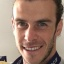
\includegraphics[scale=0.6]{25.png}\\
\textit{Sơ đồ khối hệ thống nhận dạng khuôn mặt sử dụng SVM}
\end{center}  
\par 
Sau quá trình quan sát cảm biến, thu nhận tín hiệu, số hóa thu được ảnh số. Hệ thống thực hiện tiền xử lý, phân tích, chuẩn hóa dữ liệu. Ở bước này, thực hiện lọc nhiễu, nâng cao chất lượng ảnh, chuẩn hóa kích thước ảnh. Đối với ảnh chứa khuôn mặt, hệ thống phát hiện và phân tách khuôn mặt và lấy vùng ảnh chứa khuôn mặt. Bước tiếp theo, biểu diễn ảnh thu được dưới dạng vector trong tọa độ không gian nhiều chiều, mỗi chiều biểu diễn một thuộc tính có giá trị là giá trị điểm ảnh tương ứng, vector này có được từ phép chuyển đổi ma trận dữ liệu ảnh tương ứng. \par    
\subsection{Quá trình huấn luyện}
Đầu vào của quá trình huấn luyện là tập dữ liệu các đối tượng đã được gán nhãn. Sau khi có tập dữ liệu được biểu diễn dưới dạng các vector, tiến hành trích chọn đặc trưng, biến đổi không gian biểu diễn dữ liệu đối tượng từ không gian quan sát sang không gian biểu diễn đặc trưng. Trong hệ thống nhận dạng khuôn mặt này, sử dụng phép biến đổi \textbf{PCA} để thực hiện trích chọn đặc trưng. Phép biến đổi \textbf{PCA} thực hiện trích chọn ra và giữ lại \textit{k} thành phần khác nhau nhất giữa các vector dữ liệu phục vụ hiệu quả cho quá trình học và ra quyết định phân lớp nhận dạng. Đầu vào của quá trình huấn luyện là các vector dữ liệu \textit{k} thành phần thu được từ phép biến đổi \textbf{PCA}, \textit{k} thành phần cũng là \textit{k} thuộc tính của các đối tượng dùng để đối sánh và phân lớp. Mỗi đối tượng được gán nhãn các lớp tương ứng, các vector biểu diễn cùng một đối tượng có cùng nhãn, ngược lại, các vector biểu diễn các đối tượng khác nhau có nhãn khác nhau. Bước tiếp theo tiến hành phân lớp đối tượng sử dụng \textbf{SVM}, tìm ra các mặt phân cách giữa các lớp và hàm phân tách tuyến tính các lớp. Lưu lại hàm phân lớp tìm được và ma trận phép biến đổi \textbf{PCA} trong cơ sở dữ liệu, làm cơ sở cho quá trình quyết định nhận dạng. 
\subsection{Quyết định nhận dạng} 
Đầu vào của quá trình quyết định nhận dạng là dữ liệu đối tượng cần nhận dạng. Từ ảnh chứa đối tượng cần nhận dạng, thực hiện bước tiền xử lý và biểu diễn đối tượng dưới dạng vector dữ liệu trong không gian(đây là giai đoạn chung của cả hệ thống, sử dụng cho cả quá trình huấn luyện và quá trình nhận dạng). Sau khi biểu diễn đối tượng cần nhận dạng, thực hiện phép biến đổi \textbf{PCA} để trích chọn đặc trưng, giảm số chiều của vector dữ liệu, giữ lại \textit{k} thành phần của đối tượng, sử dụng ma trận phép biến đổi \textbf{PCA} có được từ quá trình huấn luyện, được lưu trữ trong cơ sở dữ liệu, thu được vector dữ liệu \textit{k} thành phần biểu diễn \textit{k} thuộc tính của đối tượng cần nhận dạng.
Sử dụng hàm phân lớp tìm được từ quá trình huấn luyện, được lưu trữ trong cơ sở dữ liệu, đầu vào là vector dữ liệu đã thu được, quyết định nhận dạng đối tượng và đưa ra kết quả. 

\section{Cài đặt thử nghiệm}
\subsection{Môi trường cài đặt}
Chương trình được cài đặt sử dụng một số thư viện trên môi trường \textsf{Python}: \par 
\begin{itemize}
\item \textsf{matplotlib}: thư viện làm việc với đồ thị 2D của \textsf{Python}, cung cấp các module làm việc tương tự với MATLAB.
\item \textsf{numpy}: package hỗ trợ tính toán khoa học trên \textsf{Python}.
\item \textsf{scikit-learn}: thư viện học máy của \textsf{Python}, có các thuật toán phân loại, hồi quy và phân cụm,... được thiết kế tương thích với các thư viện tính toán khoa học \textsf{NumPy} và \textsf{SciPy} của \textsf{Python}.
\item \textsf{autocrop}: công cụ tự động phát hiện và cắt hình ảnh khuôn mặt từ hình ảnh ban đầu, được phát triển bởi Fracois Lablanc sử dụng \textsf{opencv}.
\end{itemize}  
\par 
Ngoài ra chương trình còn sử dụng một số thư viện \textsf{Python}, \textsf{joblib}(hỗ trợ cho việc lưu trữ dữ liệu sau quá trình trích chọn đặc trưng và học phân lớp), \textsf{tkinter}(xây dựng giao diện chương trình đơn giản),...

\subsection{Xây dựng chương trình}
Chương trình được xây dựng nhằm hai mục đích là đánh giá ảnh hưởng của \texttt{SVM} đến hệ thống nhận dạng và ứng dụng chương trình trong thực tế dành cho người dùng. Các bước thực hiện:  
\begin{itemize}
\item \textit{Thu thập tín hiệu, số hóa}
\begin{itemize}
\item Để có được số lượng ảnh đủ lớn của những người đăng ký nhận dạng, thu thập ảnh của 5 người nổi tiếng trên Internet với số lượng khác nhau, việc này đã bỏ qua bước quan sát cảm biến, thu thập tín hiệu từ camera và số hóa.  
\item Thực hiện thu thập 201 ảnh của 5 người khác nhau. Đối tượng được đăng ký nhận dạng gồm có 3 nam và 2 nữ. Mỗi người với số lượng ảnh lần lượt là 31, 56, 39, 61 và 14 ảnh. 
\end{itemize}
\item \textit{Tiền xử lý, phân tích, chuẩn hóa dữ liệu}
\begin{itemize}
\item Cần lưu ý là ảnh thu thập chỉ chứa khuôn mặt đối tượng cần đăng ký và nhận dạng, ngoài ra không chứa thêm bất kỳ khuôn mặt nào khác, do công cụ sử dụng \texttt{autocrop} chỉ làm việc với ảnh chứa một khuôn mặt. 
\item Từ các ảnh chứa đối tượng với các kích cỡ khác nhau đã thu thập, thực hiện bước phát hiện và phân tách khuôn mặt của đối tượng sử dụng công cụ \texttt{autocrop}. Kích thước ảnh chứa khuôn mặt là \texttt{64x64}, trong đó khuôn mặt chiếm 80\% chiều dọc ảnh.
\item Chuyển đổi từ ảnh màu sang ảnh đa mức xám để thuận tiện hơn trong việc tính toán và xử lý số học. Dữ liệu thu được cho mỗi ảnh là một ma trận dữ liệu kích thước \texttt{64x64}, với giá trị mỗi phần tử ma trận là giá trị hàm độ chói của ảnh tại mỗi vị trí tọa độ (x,y) trong mặt phẳng ảnh.  
\end{itemize}
\end{itemize}
Quá trình tiếp theo được chia thành 2 giai đoạn chính:
\subsubsection{Quá trình huấn luyện} 
\begin{itemize}
\item \textit{Biểu diễn, trích chọn đặc trưng}
\begin{itemize}
\item Chuyển đổi ma trận dữ liệu ảnh thành ma trận dữ liệu kích thước \texttt{1x4096}, ma trận dữ liệu mới có hình dạng 1 hàng và 4096 cột. Ma trận mới thu được là biểu diễn của một vector dữ liệu gồm 4096 thành phần tương ứng với giá trị hàm độ chói tại mỗi vị trí điển ảnh. 
\item Mỗi đối tượng được phân biệt bằng các định danh là mã số riêng dành cho đối tượng đó, hay còn gọi là nhãn. Nhãn là các số nguyên dương bắt đầu từ 0,1,2,... Gán nhãn cho các vector dữ liệu tương ứng với các đối tượng mà nó biểu diễn.   
\item Từ tập 201 ảnh dữ liệu đầu vào, xây dựng 201 vector dữ liệu biểu diễn cho các ảnh, biểu diễn tập dữ liệu đầu vào thành ma trận dữ liệu kích thước 201x4096, với mỗi hàng biểu diễn dữ liệu của mỗi ảnh, các cột là giá trị hàm độ chói của các điểm ảnh tương ứng với ảnh đó. 
\item Chọn \textit{k=120}, là số thành phần cần giữ lại, các thành phần quan trọng nhất, phân biệt nhất giữa các đối tượng. Thực hiện phép biến đổi \texttt{PCA} thu được tập dữ liệu mới với số chiều của mỗi vector chỉ còn là 120, kích thước ma trận biểu diễn tập dữ liệu thu được là \texttt{201x120} và ma trận phép biến đổi \texttt{PCA}. Lưu trữ lại ma trận phép biến đổi \texttt{PCA} vào trong file, sử dụng thư viện \texttt{joblib} của \texttt{Python}.   
\end{itemize}
\item \textit{Học phân lớp}
\begin{itemize}
\item Tập dữ liệu đầu vào của quá trình học phân lớp là tập dữ liệu các vector biểu diễn đối tượng đã được trích chọn đặc trưng, biểu diễn bởi ma trận dữ liệu kích thước \texttt{201x120}. 
\item Thực hiện quá trình học phân lớp sử dụng SVM phân lớp tuyến tính. Chọn \texttt{c=0.1}, tham số thể hiện mức độ ảnh hưởng của lỗi đến hệ thống. 
\item Lưu trữ hàm phân lớp các đối tượng tìm được trong file, sử dụng thư viện \texttt{joblib} của \texttt{Python}.  
\end{itemize}
\end{itemize}

\subsubsection{Quyết định nhận dạng}
\begin{itemize}
\item \textit{Biểu diễn, trích chọn đặc trưng}
\begin{itemize}
\item Đầu vào của quá trình nhận dạng là ảnh chứa đối tượng cần nhận dạng.
\item Chuyển đổi ma trận dữ liệu ảnh thành ma trận dữ liệu kích thước \texttt{1x4096}, ma trận dữ liệu mới có hình dạng 1 hàng và 4096 cột. Ma trận mới thu được là biểu diễn của một vector dữ liệu gồm 4096 thành phần tương ứng với giá trị hàm độ chói tại mỗi vị trí điển ảnh. 
\item Sử dụng ma trận phép biến đổi \texttt{PCA} đã tìm được và lưu trữ trong quá trình huấn luyện, biến đổi vector dữ liệu ảnh cần nhận dạng về cùng số chiều(\textit{k=120}) với mỗi vector dữ liệu huấn luyện.  
\end{itemize}
\item \textit{Quyết định nhận dạng, phân lớp}
\begin{itemize}
\item Sử dụng hàm phân lớp đã tìm được và lưu trữ trong quá trình huấn luyện, với đầu vào là vector dữ liệu ảnh chứa đối tượng cần nhận dạng đã được trích chọn đặc trưng, tiến hành phân lớp đối tượng. 
\item Kết quả thu được sau khi sử dụng hàm phân lớp đối tượng là nhãn tương ứng của đối tượng, đưa ra kết quả là đối tượng tương ứng với nhãn đó.
\end{itemize}
\end{itemize}

\subsubsection{Kiểm thử chất lượng phân lớp}
Để đánh giá độ chính xác cũng như chất lượng nhận dạng của hệ thống, chia tập dữ liệu 201 ảnh từ tập dữ liệu dùng để huấn luyện thành 2 phần: \par 
\begin{itemize}
\item Dữ liệu huấn luyện : chiếm 85\% tập dữ liệu
\item Dữ liệu nhận dạng : chiếm 15\% tập dữ liệu
\end{itemize}
\par 
Trong tập dữ liệu nhận dạng, số ảnh nhận dạng dành cho mỗi đối tượng chiếm 15\% tổng số ảnh biểu diễn đối tượng đó. Xây dựng chương trình kiểm thử có kịch bản giống với chương trình ứng dụng cho người dùng, phần khác chính là đầu vào của quá trình nhận dạng là tập các vector biểu diễn đối tượng được biểu diễn dưới dạng ma trận. Đầu ra của chương trình là ma trận lỗi(\textit{confusion matrix}), cho phép trực quan hoá hiệu suất của thuật toán và tỷ lệ độ chính xác của hệ thống. \textit{Confusion matrix} thể hiện có bao nhiêu điểm dữ liệu thực sự thuộc vào một lớp, và được dự đoán là rơi vào một lớp. \textit{Confusion matrix} là một ma trận vuông kích thước mỗi chiều bằng số lượng lớp dữ liệu. Giá trị tại cột thứ \texttt{i}, hàng thứ \texttt{j} là số lượng điểm thực tế thuộc lớp \texttt{i} nhưng lại được dự đoán là thuộc vào lớp \texttt{j}. Tổng số phần tử trong toàn ma trận này là số điểm dữ liệu trong tập kiểm thử. Các phần tử trên đường chéo của ma trận là số điểm được phân loại đúng của mỗi lớp dữ liệu. Độ chính xác của hệ thống được tính bằng tổng các phần tử trên đường chéo chia cho tổng các phần tử của toàn ma trận.  
\subsection{Chương trình ứng dụng dành cho người dùng}
Quá trình học phân lớp đã được thực hiện trong hệ thống khi thu thập đủ dữ liệu người đăng ký cần nhận dạng, vì vậy chương trình của người dùng được xây dựng sử dụng hàm phân lớp mà hệ thống đã tìm được trong quá trình huấn luyện. Chương trình đưa ra kết quả nhận dạng người trong số những người đã được đăng ký với hệ thống. Chương trình có giao diện đơn giản dành cho người dùng, cho phép người dùng lựa chọn một ảnh trong bộ ảnh kiểm thử, đã được tiền xử lý, đưa về dạng chuẩn cùng với ảnh dành cho quá trình huấn luyện. 
\begin{center}

\includegraphics[scale=0.7]{36.png}\\
\textit{Giao diện chương trình}
\end{center} 
\par 
Bộ dữ liệu dành cho người dùng kiểm thử gồm tất cả 51 ảnh của 5 đối tượng khác nhau đã được đăng ký, được chuẩn hoá, tiền xử lý đưa về dạng chuẩn.\par 
Một số kết quả sau khi người dùng lựa chọn ảnh để nhận dạng:
\begin{center}
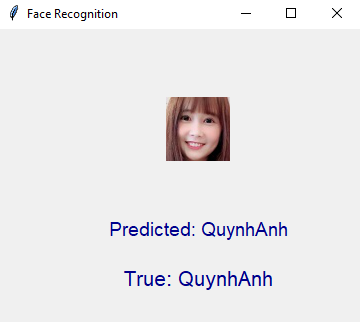
\includegraphics[scale=0.7]{4.png}\\

\includegraphics[scale=0.7]{5.png}\\

\includegraphics[scale=0.7]{6.png}\\
\end{center} 
Trong đó: 
\begin{itemize}
\item \textit{Predicted}: kết quả nhận dạng hệ thống.
\item \textit{True}: kết quả chính xác của đối tượng.
\end{itemize}   

\section{Đánh giá ảnh hưởng SVM đến hệ thống nhận dạng khuôn mặt}
\subsection{Kết quả thử nghiệm}
Chương trình kiểm thử chất lượng hệ thống cho kết quả như sau:\par  
\begin{center}
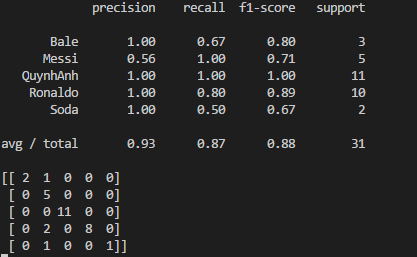
\includegraphics[scale=0.9]{11.png}\\
\textit{Kết quả thử nghiệm}\\
\end{center}
Các thông số: \par 
\begin{itemize}
\item \textit{support:} số vector dữ liệu được phân lớp vào lớp đó. 
\item \textit{precision:} tỷ lệ số vector dữ liệu phân lớp đúng trên tổng số vector dữ liệu được phân loại vào lớp đó.
\item \textit{recall:} tỷ lệ số vector dữ liệu phân lớp đúng trên tổng số vector dữ liệu của đối tượng đó.
\item \textit{f1-score:} trung bình điều hoà(\textit{harmonic mean}) của các tiêu chí \textit{precision} và \textit{recall}, $\mathit{F_1}$ càng cao, bộ phân lớp càng tốt: \par 
\begin{center}
{\fontsize{18pt}{1}\selectfont $\mathit{F_1 = 2\frac{precision*recall}{precision+recall} }$}\\
\end{center}  
\end{itemize} 
 
\noindent \textbf{Nhận xét:}
\begin{itemize}
\item Độ chính xác của hệ thống \texttt{0.88}, tương đối tốt. 
\end{itemize}
\subsection{Phân tích ảnh hưởng SVM đến chất lượng hệ thống nhận dạng khuôn mặt}
Đối với tập dữ liệu học không đồng đều, tức là với mỗi đối tượng, số lượng mẫu biểu diễn người đó khác nhau, chất lượng phân lớp tốt hơn đối với các đối tượng có tập dữ liệu học đủ lớn, đối tượng có tập dữ liệu học nhỏ cho kết quả phân lớp chưa tốt. Để kiểm thử ảnh hưởng số lượng vector dữ liệu học của mỗi đối tượng, thực hiện chọn bộ dữ liệu kiểm thử 10 ảnh trên mỗi đối tượng được lấy từ tập dữ liệu 201 ảnh ban đầu, vậy số ảnh dùng cho quá trình huấn luyện của các đối tượng sẽ giảm đi 10 ảnh, lần lượt là 21, 46, 29, 51 và 4 ảnh. Áp dụng quy trình kiểm thử chất lượng đã nêu trên, thu được kết quả: \par 
\begin{center}

\includegraphics[scale=0.9]{35.png}
\end{center}
\par 

Kết quả thu được cho thấy, với 4 đối tượng đầu tiên, chất lượng phân lớp tương đối tốt, đối tượng cuối cùng cho chất lượng phân lớp chưa tốt. Với đối tượng có số ảnh dùng cho việc huấn luyện đủ lớn, giúp cho việc chọn các vector hỗ trợ càng tốt hơn, vì số lượng các vector càng lớn thì càng có nhiều lựa chọn và tìm ra vector hỗ trợ tốt nhất để phân tách giữa các lớp, nói cách khác, vùng không gian dành cho lớp đó có thể sẽ càng lớn và vì vậy xác xuất để phân lớp đúng đối tượng đó sẽ càng lớn. Ngược lại, đối tượng có số ảnh dùng cho việc huấn luyện nhỏ, số lượng các vector biểu diễn dữ liệu nhỏ, vì vậy vector hỗ trợ tìm được có thể chưa tốt ảnh hưởng đến việc tìm ra mặt phân tách giữa các lớp, vùng không gian biểu diễn cho đối tượng có thể nhỏ hoặc được xác định không chính xác với đối tượng đó, ảnh hưởng tới hệ thộng nhận dạng. Trong tập dữ liệu huấn luyện cho đối tượng này, có thể chứa các vector dữ liệu lỗi, mà số lượng vector dữ liệu biểu diễn đối tượng nhỏ, vì thế không thể nhận biết được đó có phải vector dữ liệu lỗi so với các vector dữ liệu khác của đối tượng đó hay không, do đó ảnh hưởng xấu đến chất lượng phân lớp. \par 
Trong số 4 đối tượng đầu tiên, đối tượng thứ 3(có số ảnh huấn luyện là 29) cho chất lượng tốt nhất. Số lượng ảnh dùng cho quá trình huấn luyện không phải là nhiều nhất nhưng có thể thấy các vector phân bố không quá dày đặc mà trải ra làm cho vùng không gian mô tả đối tượng lớn hơn, vector hỗ trợ được chọn có thể phân lớp tốt hơn đối tượng đó, do đó xác xuất để phân lớp đúng vào lớp đó càng lớn, độ chính xác càng cao. Người thứ tư có số lượng ảnh dùng cho huấn luyện là lớn nhất nhưng lại không cho chất lượng tốt nhất, có thể lý giải rằng tập dữ liệu biểu diễn người này có thể dày đặc, việc chọn vector hỗ trợ có thể không tốt bằng người thứ ba, nói cách khác, số dữ liệu học chưa biểu diễn hết được đối tượng này, do đó, vùng không gian dành cho đối tượng này chưa đủ lớn hơn vùng không gian dành cho đối tượng có ít dữ liệu học hơn, cho nên xác xuất phân lớp đúng vào lớp này là nhỏ hơn lớp thứ ba.\par 
Vậy chất lượng hệ thống nhận dạng phụ thuộc vào \textit{SVM}, vector hỗ trợ phân tách các lớp càng tốt thì chất lượng hệ thống nhận dạng khuôn mặt càng đạt độ chính xác cao. \par 

\newpage
\section{Kết luận}
\textit{Support Vector Machine} là một phương pháp học có giám sát, mục đích chính của SVM là đi tìm mặt phân cách sao cho mức lề tìm được là lớn nhất, đồng nghĩa với việc các điểm dữ liệu là an toàn nhất so với mặt phân cách(được phân lớp tốt nhất). Phương pháp SVM giải quyết được bài toán lỗi xảy ra ở một vài điểm dữ liệu, tối ưu được hàm mất mát do lỗi gây ra, cho chất lượng phân lớp tốt đối với tập dữ liệu chứa lỗi. Trong hệ thống nhận dạng, SVM đóng vai trò học phân lớp và quyết định nhận dạng, kết hợp với phương pháp PCA, SVM cho tốc độ phân lớp và hiệu quả cao trong quyết định nhận dạng và đưa ra kết quả. SVM ảnh hưởng trực tiếp đến chất lượng hệ thống nhận dạng khuôn mặt, SVM tìm được phụ thuộc vào tập dữ liệu huấn luyện đầu vào, do đó, tập dữ liệu huấn luyện tốt sẽ cho kết quả phân lớp cũng như quyết định nhận dạng có độ chính xác cao.       
      
\newpage
\section{Tài liệu tham khảo}
\begin{enumerate}
\item Ján Mazanec, Martin Melisek, Milos Oravec, Jarmila Pavlovicova - Support Vector Machine, PCA and LDA in Face Recognition - Vol. 59, No. 4, 2008, 203-209 - Journal of ELECTRICAL ENGINEERING.
\item Christopher M. Bishop - Pattern Recognition and Machine Learning - 2006 Springer Science+Business Media, LLC
\item Hongjun Jia and Aleix M. Martinez - Support Vector Machines in Face Recognition with Occlusions - The Ohio State University, Columbus, OH 43210, USA.
\item Jan Kremer, Kim Steenstrup Pedersen, Christian Igel - Active Learning with Support Vector Machines.

\item \href{url}{https://scikit-learn.org/stable/modules/svm.html}
\item \href{url}{https://scikit-learn.org/stable/modules/generated/sklearn.svm.SVC.html\#sklearn.svm.SVC}
\item \href{url}{https://scikit-learn.org/stable/auto\_examples/applications/plot\_face\_recognition.html\#sphx-glr-auto-examples-applications-plot-face-recognition-py}

\end{enumerate}    
\end{document}